%%____________________________________________________________________ 
%% File: CreatingProjects.tex
%%____________________________________________________________________ 
%%  
%% Author: Shaun ASHBY <Shaun.Ashby@cern.ch>
%% Update: 2005-11-02 17:05:54+0100
%% Revision: $Id: CreatingProjects.tex,v 1.6.2.1 2007/03/02 13:54:00 sashby Exp $ 
%%
%% Copyright: 2005 (C) Shaun ASHBY
%%
%%--------------------------------------------------------------------
\chapter{Creating SCRAM-Managed Projects}\label{ch:creatingprojects}
\index{SCRAM!creating projects}
\index{creating SCRAM projects}

A \scram\ project is a releasable unit covering a particular software
domain, for example an analysis framework, event simulation or reconstruction.
Libraries and binary executables are the typical basic build products and these
can have separate storage areas. A configuration directory contains all the
files necessary to allow \scram\ to configure a dedicated project
release area for a version of the project. External requirements are
configured automatically. 
The structure of a project can be freely chosen since \scram\ does not
impose restrictions on project structure: it is
easy to modify \scram\ build behaviour according to site conventions.

\ni Generally, a project is subdivided into \texttt{subsystems} and
\texttt{packages} according to the tree structure of the source code
directory. Dependencies are expressed in terms of packages
where a package is typically built into a shared library: in fact,
the build products that correspond to a certain set of source files in
a certain location can be freely modified to suit the project. 
The principal reason for assuming (or enforcing in some cases) that
packages map to libraries is to enable proper dependency tracking and
automatic ordering of build operations. From Version 1.0 of \scram, 
this feature is fully supported both internally (to establish correct library
ordering in linker information) and via \texttt{gmake} which controls
the build ordering once the dependency information is correctly
obtained by \scram.

\ni Source files and header files have separate directories appearing under
\texttt{src} and \texttt{interface} or \texttt{include} respectively.
An additional directory called \texttt{test} can be used as a location 
to build binary executables for testing. Likewise, other directories 
can be used as locations to define other build products, for example 
\texttt{bin} or \texttt{app} for binary executables and applications 
which should be released as project deliverables.

\begin{figure}[htb]\index{project structure!recommended}
  \begin{center}
    \leavevmode 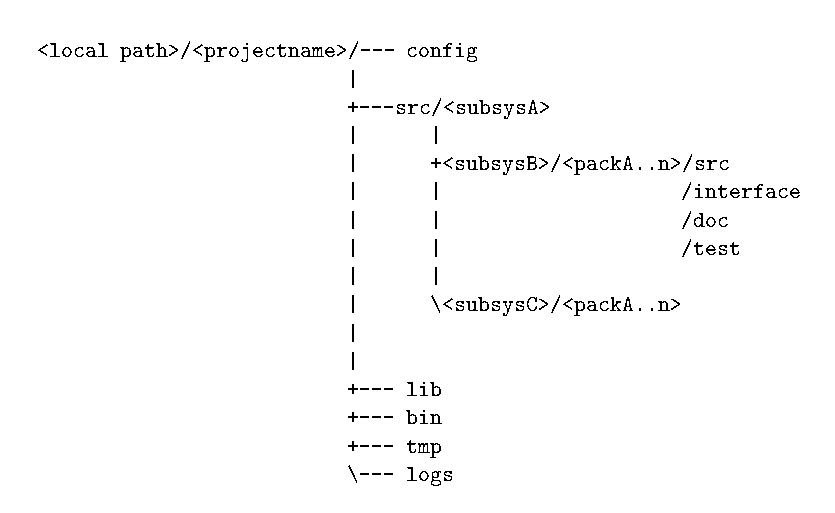
\epsfig{file=images/projectstructure.eps, width=\linewidth}
    \caption{Recommended \scram\ project structure. The directories
      \texttt{tmp} and \texttt{logs} are created
      automatically and directories for build products 
      like \texttt{lib} and \texttt{bin} 
      are created as appropriate given instructions 
      read from a project build file.}
    \label{fig:recprojstruct} 
  \end{center}
\end{figure}

\ni The corresponding \scram\ project structure consists of a directory
tree like that shown in Figure~\ref{fig:recprojstruct}.

\ni This chapter describes some of the important internal configuration aspects of
\scram\ that are used to define projects and should provide all the
information required for administrators and developers alike to
configure a \scram-managed project.

\section{SCRAM Project Components}

Every \scram\ project has documents to describe it and a code
repository from where these documents, and project source code, can be
accessed using a version management system.
The two elements are described in the following sections.

\subsection{Configuration Documents}\label{sec:scramconfigdocs}
\index{SCRAM!project configuration files}

\ni There are two types of project areas:
\begin{itemize}
\item \texttt{Releases} which are normally installed in a central location.
\item \texttt{Developer Areas} which are areas that are cloned from
  centrally installed releases but allow private access for software 
  development with the same controlled configuration as the release.
\end{itemize}

\ni The processes for initialising areas in each of these cases is different.
Each project must have a unique version, a name and a tool
configuration from which interfaces to external software can be
established. These interfaces express external dependencies in the
same way as individual packages in the project or release area of the
project. Their definitions are contained inside a toolbox and
list all settings needed by the \scram\ build or runtime environments (for
example, \texttt{INCLUDE} paths, libraries provided by the tools or \texttt{PATH} elements
which should be added to the user environment).

\ni Configuration instructions for \scram\ are passed using documents called
\texttt{ActiveDocs} which are \texttt{XML} files (the support for
\texttt{XML} document parsing is a new feature in this release).
These are web-enabled mark-up documents, each being associated with a
download and cacheing mechanism that is accessed using a \texttt{URL}. This
\texttt{URL} can behave like a normal \texttt{WWW} \texttt{URL} or can be a file or a
path to a \texttt{CVS} server. A number of \texttt{ActiveDoc} markup tags are
defined, some of which are common to all types of document; some tags
are specific for their application and only used in a particular class
of document.  An \texttt{ActiveDoc} document must begin with a special
statement that informs \scram\ what sort of document it is and how it
should be parsed; each type of statement is specific to a class of
functionality. The parent tag
\begin{tagprint}
  \lbkt\texttt{doc} type=\textit{"type"} version=\textit{"version"}\rbkt
\end{tagprint}
\ni is always the first line of the document after the \texttt{XML}
document header
\begin{tagprint}
  \xmldocheader
\end{tagprint}

\ni The \texttt{doc} type is set according to the \scram\ parsing
class and all \scram\ \texttt{XML} documents must end with a corresponding
\lbkt$/$\texttt{doc}\rbkt tag.

\ni There are three main different classes of \texttt{ActiveDoc} document
that are needed to configure a project: \texttt{BootStrapProject},
\texttt{RequirementsDoc} and \texttt{ToolDoc}. These classes are
described next.

\subsubsection{The BootStrapProject Class}\label{sec:bootstrapclass}
\index{\texttt{BootStrapProject} class}
A single document describes how the project should be structured and
which tools should be configured. Usually referred to as a \texttt{bootstrap} file, it must start with
the statement\index{project \texttt{BootStrapFile}} 
\index{bootstrap file}
\begin{tagprint}
  \lbkt\texttt{doc} type=\texttt{"Configuration::BootStrapProject"}
  version=\textit{"1.0"}\rbkt
\end{tagprint}
\ni The name of this file is completely arbitrary. The function of
the bootstrap document is to define the name and version of a project
and to tell \scram\ from where it can download the configuration and
source code files, and where to put them inside the project release
area. There must be a bootstrap file in every \scram\ project.

\ni The markup tags specify a path to a \texttt{CVS} server, the name of the
project requirements document and the location of the project
configuration directory within the project area.  The available markup
tags are as follows--
\index{\texttt{BootStrapProject} markup tags}
\index{\texttt{BootStrapFile} markup tags} 
\begin{description}
\item[\lbkt\texttt{project} name=\textit{"name"} version=\textit{"version"}\rbkt~\tagend{project}]\mbox{}\\
  Specify the name an version of the project. The version should be a
  valid \texttt{CVS} symbolic tag which must exist on all files in the
  configuration directory and the project source code. Explanatory
  text can be put between the \lbkt\texttt{project}\dots\rbkt tags: this
  text will be printed to the screen when bootstrapping the project.
\item[\lbkt\texttt{config} dir=\textit{"dirname"}$/$\rbkt]\mbox{}\\
  Specify the name of a directory relative to the top of the project
  area where the configuration files can be found.
\item[\lbkt\texttt{base} url=\textit{"baseurl"}\rbkt~\tagend{base}]\mbox{}\\
  A common element in multiple \texttt{URL}s, such as a \texttt{CVS} server name, is
  supplied using the base tag. The \texttt{URL} type can be \texttt{cvs:}
  (using a \texttt{CVS} repository) or \texttt{file:} (a standalone file). Any
  \texttt{URL} specified between the start and end base tags will be merged
  with the \texttt{URL} \textit{baseurl} according to the following merge
  rules:
  \begin{itemize}
  \item A merge will only take place if the \texttt{URL} and \textit{baseurl}
    types match, \eg both have type \texttt{cvs:} or \texttt{file:}
  \item The base server name is taken if it isn't already defined
  \item The \textit{baseurl} path is prepended to any \texttt{URL} specified
  \item Variables provided in the base parameter list are only added
    if not already defined, \eg definition of the directory name when
    downloading the configuration files
  \end{itemize}
\item[\lbkt\texttt{download} url=\textit{"url"} name=\textit{"dirname"}$/$\rbkt]\mbox{}\\
  Each \texttt{URL} will be merged with the base \texttt{URL} defined in a
  \tagstart{base} tag and treated as a download location which is
  passed to \texttt{CVS} for checking out files from a repository. The name of
  the destination directory will be \textit{dirname}, and will be
  located relative to the top of the project area.
\item[\lbkt\texttt{requirementsdoc} name=\textit{"docname"}$/$\rbkt]\mbox{}\\
  Specify the name of the project requirements document. The path is
  relative to the top of the project area.
\end{description}

\subsubsection{The RequirementsDoc Class}\label{sec:requirementsdocclass}
\index{\texttt{RequirementsDoc} class}

To make external products available in a project area and be able to
link against external libraries, a requirements file is used. This
file starts with the statement\index{requirements file}
\begin{tagprint}
  \lbkt\texttt{doc} type=\texttt{"BuildSystem::Requirements"}
  version=\textit{"2.0"}\rbkt
\end{tagprint}
\ni and specifies the external tools and their corresponding versions
that should be configured. The requirements file provides information
for \scram\ to use when downloading the tool descriptions from the
toolbox \texttt{CVS} repository. If more than one version of a tool is defined,
the first one is taken as the default.
The following tags are available:

\begin{description}     
\item[\lbkt\texttt{require} name=\textit{"name"} version=\textit{"version"} url=\textit{"url"}$/$\rbkt]\mbox{}\\
  Specify the name and version of a required tool. The \texttt{URL} should
  point to a \texttt{ToolDoc} that describes the tool. Base \texttt{URL} tags
  (\lbkt\texttt{base}\rbkt\ldots) can be used to modify the \texttt{URL}.
\item[\lbkt\texttt{include} url=\textit{"url"}$/$\rbkt]\mbox{}\\
  This is for \texttt{URL} document preprocessing.\texttt{ActiveDocs} provide
  an equivalent of the \texttt{C}-preprocessor
  \texttt{\#include}
  \index{\texttt{include} directive}
  directive that is web-aware. In this way, it is possible to assemble
  a document from many components that are maintained at different
  locations.  A common configuration file containing multiple tool
  \lbkt\texttt{require}\rbkt statements can be included in this way.
\item[\lbkt\texttt{architecture} name=\textit{"arch"}\rbkt~\tagend{architecture}]\mbox{}\\
\index{architecture tags}
\index{SCRAM!architecture}
\index{\texttt{SCRAM\_ARCH}}
  \ni The \textit{arch} is an architecture tag which limits certain
  functionality only to a specific operating system. This
  architecture is determined automatically by \scram. Unlike previous
  versions, the mechanism to determine the architecture name is
  defined in \texttt{Installation/SCRAM\_SITE.pm} and is fully
  customisable. Internally, \scram\ sets a variable called \texttt{SCRAM\_ARCH} to
  whatever is determined as the architecture string. This string can
  then be used as \textit{arch} (either the full architecture name or an
  abbreviation will match).

\item[\lbkt\texttt{download} url=\textit{"url"}$/$\rbkt]\mbox{}\\
  Specify a link to download information for the tool.
\item[\lbkt\texttt{select} name=\textit{"name"}$/$\rbkt]\mbox{}\\
  Select a tool from a list of available tools.
\end{description}

\subsubsection{The ToolDoc Class}\label{sec:tooldocclass}
\index{\texttt{ToolDoc}!class}
An external tool is described using a tool description file called a
\texttt{ToolDoc}. When a tool is required, a certain version of that
tool is configured by \scram\ in the project area.  A tool description
begins with the statement\index{\texttt{ToolDoc}}
\begin{tagprint}
  \lbkt\texttt{doc} type=\texttt{"BuildSystem::ToolDoc"} version=\textit{"1.0"}\rbkt
\end{tagprint}
\ni The \texttt{ToolDoc} describes such things as the default location
of the tool on the system, the names of libraries to be used when
linking against the tool and environment variables that must be set at
runtime. The external dependencies of the tool are also declared.

\ni The following tags are available in \texttt{ToolDoc}s:
\index{\texttt{ToolDoc}!valid markup tags}
\begin{description}     
\item[\lbkt\texttt{tool} name=\textit{"name"} version=\textit{"version"}\rbkt\tagend{tool}]\mbox{}\\
  Specify the name and the version of the tool that is being
  described. Everything between these tags relates to version
  \textit{version} of the tool.
\item[\mbox{\lbkt\texttt{environment} name=\textit{"variable"}
    {[}default=`\textit{"def"}' \textbf{or} value=`\textit{"value"}'{]}
    type=\textit{"type"}$/$\rbkt}]
  Set up a variable in the \scram\ environment for this tool.
  Either `value' or `default' can be set
  to provide the appropriate path for the variable but not both.
\item[\mbox{\lbkt\texttt{runtime} name=\textit{"variable"}
    {[}type=`\textit{"path"}'{]}
    {[}handler=`\textit{"warn","error"}'{]} $/$\rbkt}]\mbox{}\\
  Define a runtime variable which should be set in the users' shell
  environment. The optional variable type \textit{type} can be set
  to \texttt{path} for a path-like variable, \eg
  \texttt{\$PATH} or \texttt{\$LD\_LIBRARY\_PATH}, at runtime.
  If the handler option \textit{handler} is set to \texttt{warn},
  \scram\ will not pause and prompt for a value for the runtime
  variable if the value is incorrect (for example, if the path is
  missing because the directory has not yet been created).
\item[\lbkt\texttt{use} name=\textit{"tool name"}$/$\rbkt]\mbox{}\\
  Specify that the tool has a dependency on another external tool.
\item[\lbkt\texttt{lib} name=\textit{"libname"}$/$\rbkt]\mbox{}\\
  Specify the name of a library belonging to the tool. Note that the
  preceding `lib' or extension are not required.
\item[\tagstart{client}~\tagend{client}]\mbox{}\\
  Any \inbrackets{environment} definition between these tags will be
  checked as a directory location on the client machine.
  The presence of all libraries defined by \lbkt\texttt{lib}\rbkt tags 
  will be checked for automatically. The \texttt{client} tags should
  only contain \texttt{environment} tags: if an environment is
  architecture-specific, the \texttt{client} block must be included in
  the architecture block and not the other way around.
\item[\tagstart{makefile}~\tagend{makefile}]\mbox{}\\
  These tags delimit \texttt{gmake} makefile content intended for
  inclusion in the build system associated with the tool. It is preferable to use
  text templates (or modify existing templates) if the content to be
  added is more than a single line (\eg a variable definition).
\item[\lbkt\texttt{flags} \texttt{NAME}="definition"\rbkt]\mbox{}\\
  Extra compiler flags can be specified which will be added to the
  global compiler flags if the tool defining them is required
  globally, or added to the compiler flags for a package if the tool
  is required there.
\end{description}

\ni Note that all environment variables can be referred to by others in
addition to internal \scram\ variables like \texttt{\$SCRAM\_ARCH}, the
tool name \texttt{\$SCRAMtoolname} and the version
\texttt{\$SCRAMtoolversion}.

\subsection{The CVS Infrastructure}\label{sec:configuringCVSinf}
\index{CVS repositories}
\index{CVS repositories!setting up for a new project}
All code management within \scram\ uses \texttt{CVS}, a versioning system 
derived from \texttt{RCS}.\footnote{However, \scram\ does
not fully depend on CVS: another tool could be used instead if
required at a later date.}
Every project consists of source code and \scram\ project
configuration files which are imported into a \texttt{CVS} repository which
has a directory structure mirroring the structure of the project itself.
\begin{figure}[ht]\index{CVS repositories!recommended structure}\index{CVSROOT}
  \begin{center}
    \leavevmode 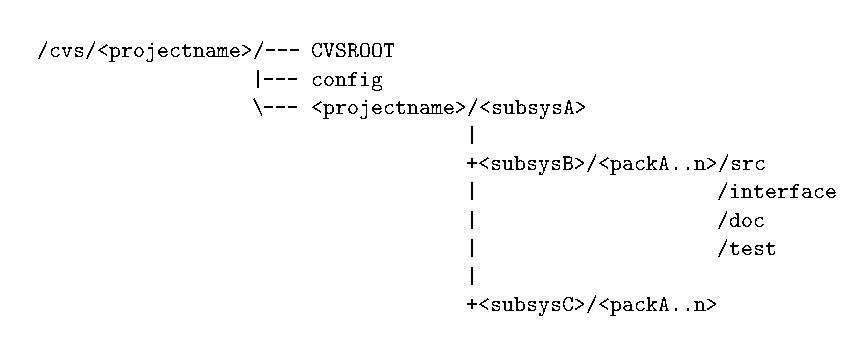
\epsfig{file=images/projectCVSstructure.eps, width=\linewidth}
    \caption{Recommended CVS repository structure for a \scram\
      project. The directory \texttt{CVSROOT} contains CVS information
      and is created automatically when initialising the CVS repository.}
    \label{fig:recprojstructCVS}
  \end{center}
\end{figure}
The typical repository structure, based on the project structure
described earlier, is illustrated in Figure~\ref{fig:recprojstructCVS}.
%
\subsubsection{CVS Authentication}\label{sec:CVSauth}
\index{CVSROOT!authentication settings and}
\index{CVS authentication options}
To access the CVS repository, an authentication method must be chosen
and specified in the \texttt{CVSROOT} environment variable. There are
currently two supported methods for file checkout in \scram:
\texttt{pserver:}, standard anonymous checkout, and \texttt{local:},
using a CVS repository on a local filesystem on the current machine
rather than a dedicated server accessible only via a network
connection. 

\subsubsection{Importing the Code for New Projects}\label{sec:importingcode}
\index{CVS repositories!importing files to}
\ni Moving source code into a repository when creating a new project
is explained in detail in the CVS manual but a brief description is
given here. Once project source code exists in a suitable directory tree, the
whole project can be imported into a CVS repository using 
the \texttt{cvs import} command. Initially, the \texttt{CVSROOT}
environment variable must be set and
the repository created using the command \texttt{cvs init}.
To make life easier when defining download paths in bootstrap
files, the \texttt{CVSROOT} for project \texttt{MyProject} on a local
filesystem would look like

\begin{list}{}
\item\texttt{/local/path/cvs\_repository/MyProject} 
\end{list}

\ni and would be set before importing the code. Import the
configuration directory (and contents) first

\begin{indentprint}\texttt{cd config}\end{indentprint}
\vspace{-3mm}
\begin{indentprint}
  \texttt{cvs import -m "First import of my project config" config V1-0 V1-0}
\end{indentprint}

\ni and then repeat this step for the project sources:

\begin{indentprint}\texttt{cd MyProject}\end{indentprint}
\vspace{-3mm}
\begin{indentprint}
  \texttt{cvs import -m "First import of my project src" MyProject V1-0 V1-0}
\end{indentprint}

\ni Once this has been done and assuming that the import was
successful, the original sources can be removed and then restored from \texttt{CVS}
using \texttt{cvs co MyProject}.

\subsection{The SCRAM Toolbox}\label{sec:toolboxrep}
\index{SCRAM!toolbox CVS repository}
\index{CVS repositories!for tool descriptions}
A separate \texttt{CVS} repository must exist which contains 
documents describing external tools: these are components of a {\em toolbox}. 
This is referred to as the \scram\ toolbox.
Each tool has a \texttt{ToolDoc} in which every
version of the tool that can be used in a project environment is
described. Any environment or makefile variable needed to use the
external software is declared in the file and interpreted by \scram\ as
a variable to be set up when creating the project area for the first
time, or installing a new version of the tool into an existing area.
A global configuration file (called
`the configuration') indicates which tools and the corresponding versions that can
be downloaded by \scram\ and used in project-space. The toolbox is
tagged with a \texttt{CVS} symbolic tag which is used to \textit{freeze} the
configuration: this tag is then specified in the project
\texttt{RequirementsDoc} as the version to download.
There is no requirement for a particular structure for the toolbox 
but including at least the following is recommended:

\begin{description}
\item[\textbf{Compiler Tools}]\mbox{}\\
  Any number of programming languages can be supported (for example \texttt{C},
  \texttt{C++}, \texttt{Java} or \texttt{Fortran}). The top-level
  \texttt{BuildFile} for the project should select the compilers that should
  be configured globally (compilers can also be selected for use only at
  the package level where they are required).
\item[\textbf{External Software}]\mbox{}\\
  Each external software package to be used by a project should have a
  unique tool description file which defines the required version of
  the tool.
\item[\textbf{Project Software Releases}]\mbox{}\\
  Tool descriptions for all projects that provide libraries to be used
  by other projects or tools should be created.
\item[\textbf{A Configuration File}]\mbox{}\\
  The most important element in the toolbox. The 
  configuration describes the available tools and 
  versions of these tools that are to be used in a
  project area.
\end{description}

\section{Creating a Project Release Area}\label{sec:creatProjArea}
\index{Project areas!creating new}

The starting point in a software development cycle is to create a project
release to estabish a baseline for further development. 
A \scram\ project must have, at least, the following configuration
files in a configuration directory to properly define the project:
\begin{description}
\item[\texttt{boot.xml}]\mbox{}\\
  For bootstrapping the project. This will relate a specific project
  version with the relevant source code version and define a
  requirements file to be read to select external products.
\item[\texttt{requirements.xml}]\mbox{}\\
  The requirements file containing information to be passed to the
  configuration manager for setting up external tools. A \texttt{CVS}
  symbolic tag for a released configuration specifies which tools and
  version should be downloaded from the toolbox repository.
\item[\texttt{config/BuildFile.xml}]\mbox{}\\
  The top-level \texttt{BuildFile}, containing project-wide default settings for
  export of external tools, build product storage and global compiler settings. 
\end{description}

\ni These files are normally kept in a directory called
\index{\texttt{config} directory}
\index{project configuration directory}
\texttt{config} (the name of the directory can be changed using a
directive in the boot file).  A \scram\ command exists
which can be used to grab basic template files for a new project.
Typing

\begin{scramcmd}{project -template}\end{scramcmd}

\ni will download some basic project configuration files to a
directory called \texttt{config} in the current directory. These
should be edited to suit and imported into the project CVS repository
(see Section~\ref{sec:configuringCVSinf}). Once these configuration
files exist, they must be tagged with a \texttt{CVS} symbolic tag that matches the name
and version of the project (for example \texttt{myProject\_1\_0}).
All project source code must have the same global \texttt{CVS} tag (this is
especially important if you want the bootstrap mechanism to also
download source code).

\ni Creating the project area is very easy- just type the command

\begin{scramcmd}{project -b config/boot.xml}\end{scramcmd}

\ni indicating the location of the bootstrap file after the \texttt{-b} 
option, and that's it. \scram\ will set up the tools automatically
using the settings in the default lookup file \texttt{tools-X.conf}
found in \texttt{config/site}, or whichever lookup file is
specified on the command line.

\ni Two subdirectories are created in the project area as part of the
initialisation: \texttt{config} and \texttt{.SCRAM}. All files used
for bootstrapping and the build system are contained in
\texttt{config}, downloaded directly from the \texttt{CVS} repository. The
important project information is contained in the \texttt{.SCRAM}
subdirectory
\label{sec:dotSCRAMcontents}
\index{\texttt{.SCRAM} directory} so this must not be renamed or
deleted. A closer look at the contents of the \texttt{.SCRAM}
directory reveals the following subdirectories and files:

\small{
\begin{verbatim}
 ObjectDB/
 Environment
 cache/
 InstalledTools/
 slc3_ia32_gcc323/
 DirCache.db
\end{verbatim}
}\normalsize

\ni The directories \texttt{ObjectDB}, \texttt{cache} and
\texttt{InstalledTools} store tool description files as they are downloaded
from the \texttt{CVS} repository prior to being parsed by the setup mechanism.
Once each tool has been configured for use in the current environment,
the tool information is stored in the tool cache in
a directory for the architecture (in this example,
the architecture is \texttt{slc3\_ia32\_gcc323}). The file
\texttt{Environment} contains information required about the project
by \scram. The file content for a typical project \texttt{TEST} version 
\texttt{TEST\_1\_0} looks like this: 

\small{
\begin{verbatim}
SCRAM_PROJECTNAME=TESTING
SCRAM_PROJECTVERSION=1.0
SCRAM_TOOLBOXVERSION=CMS_145a_2
SCRAM_PROJECT_TIMESTAMP=Wed-28-Feb-2007 14:10:22
LOCALTOP=/home/t/work/projects/TESTING_1.0
\end{verbatim}}\normalsize 
%
\ni These entries are also defined as environment variables, visible in
the runtime and build environments. There will also be content like
\index{\texttt{RELEASETOP} settings}
\small{
\begin{verbatim}
RELEASETOP=/home/t/work/releases/TESTING_1.0
SCRAM_PROJECT_RELEASE_TIMESTAMP=Tues-27-Feb-2007 16:12:28
\end{verbatim}
}\normalsize

\ni in a developer area, informing \scram\ that the central area containing libraries and
header files should be used first, before any of the contents of the
current area. The timestamp of the release is also shown.

\ni The file \texttt{DirCache.db} is the timestamp cache file and
contains timestamp information for each file and directory in the
project source tree and configuration directory (\texttt{config}).
This will only exist when a build has run for the project.

\subsection{The Project Boot Process}
The principle of both the bootstrapping and tool setup is the same as
with previous versions of \scram. However, in the current version there is a fundamental
difference in the way that the tool data, before and after being set
up, is stored in the project.
All tool data is now cached in a file called \texttt{ToolCache.db} which is
stored in an architecture-dependent location inside the 
project (\ie under \texttt{.SCRAM/\$SCRAM\_ARCH}).

\begin{description}
\item[Tool downloading:]\mbox{}\\ 
  After tools have been downloaded to the local \scram\ cache (usually
  \texttt{.SCRAM/cache}), those tools selected in the \texttt{RequirementsDoc} will be
  set up. For each tool, a file \texttt{.SCRAM/InstalledTools/}\textit{toolname} will
  be created. At the same time, the contents of this file will be
  parsed and stored in the tool cache file. The order in which the
  \lbkt\texttt{select}\rbkt statements appear in the \texttt{RequirementsDoc} will be the order
  in which the tools are set up \textit{and} the order in which they appear in
  any path-like runtime variables. This is completely independent of the
  order in which tool files are downloaded (that is, the order in
  which the \lbkt\texttt{require}\rbkt statements appear in the tool
  configuration file, \ie \texttt{CMSconfiguration}).
  
\item[Tool Storage:]\mbox{}\\ 
  The cache file \texttt{ToolCache.db} replaces the numerous \texttt{*.dat} files that were previously
  located in the architecture-dependent directories under \texttt{.SCRAM}. 

\item[Tool Parse:]\mbox{}\\ Once the tool is parsed and set up (using input from
  \texttt{tools-CERN.conf}), a \texttt{ToolData} object holds the
  data within the cache. The tool object provides the methods to access the
  tool metadata.

%% Skip this part for now, since it's not particularly reliable!
%%
% \item[Other Project Setup:]\mbox{}\\
%   Setting up a project area which depends on another SCRAM-managed
%   project is now quicker and less prone to error since the entire tool
%   setup is copied to the new area. Only additional tools are set up in
%   the traditional way. Note that the SCRAM projects used in the
%   current project configuration must be installed in the scram database.
%%
\end{description}

\subsection{Standalone Project Areas}

Project areas can also be bootstrapped without having access to a
\texttt{CVS} repository or a version control system by using only local copies of the project
configuration files (and toolbox files, if required). This is ideal for fast prototyping.
There are two possible methods:

\begin{description}
\item[Method 1:]\mbox{}\\ 
Use a standalone configuration directory which be copied directly to
the new project area, with \texttt{CVS} used only in the requirements
file to specify where the tool configuration and tools should be
downloaded from.
In this context, "standalone" means that the download \texttt{URL} is
of type \texttt{file:}, rather than \texttt{cvs:}.
The requirements file does specify \texttt{cvs:} with the path to the
toolbox repository.

\item[Method 2:]\mbox{}\\ 
Use a standalone configuration directory and toolbox. Both the config
and the toolbox are normal directories on a local filesystem and only
the \texttt{file:} type of \texttt{URL} is used.
\end{description}

\ni Examples of the content of boot files, requirements files and a
standalone toolbox are given in Chapter~\ref{ch:examples}.

\section{Creating a Developer Area}\label{sec:SCRAMdevareas}
\index{using SCRAM developer areas}
\index{SCRAM developer area}

\ni A developer area is an isolated area where a developer can work on a
given project without affecting other developers. This area is
associated with a particular version of a project available centrally
from which it can use resources (\eg \texttt{\#include} files, libraries or
environment files and settings). Software developers can check out source code 
from \texttt{CVS} and \scram\ will build the products defined locally
and use these in place of those available in the
central release. All other products are transparently taken from the central project
release.

\ni To develop on a given project a copy of the project must be installed
at the developer site. Available projects can be viewed using the
command \texttt{scram list}. To create the developer space, the command

\begin{scramcmd}{project}
  \inbrackets{project\_name}~\inbrackets{project\_version}
\end{scramcmd}

\ni should be issued. The project name and version above are taken
from the list of \scram\ projects. The development area has the
structure and the same build environment as the base project.
Alternatively, a developer can bootstrap a project by first
checking out the \texttt{config} directory that matches the version of
the project that the developer are is to be based on and following the
steps described in Section~\ref{sec:creatProjArea}.
This can be implemented via a web interface such that a
source code distribution of the project can be obtained via a \scram\
download mechanism which can be enabled using any web browser. Follow
the instructions in Section~\ref{sec:webbootstrap} on page 
p\pageref{sec:webbootstrap} to do this. Once
correctly configured, a project can be installed using a single-click
operation in a browser window. 

\subsection{Using the Developer Area}\label{sec:usingscramdevarea}
\index{SCRAM developer area!using a}

Once the area has been created, the \texttt{src} directory can be
populated with the source code of interest. This step
involves \texttt{CVS} alone; usually, a module corresponds to a package and so
the whole module would be checked out from the \texttt{CVS} repository. This
would be achieved using the command

\texttt{cd src;}~\texttt{cvs co}~\textit{module}

\ni Note that the above command will check out the development
\texttt{HEAD}. To check out a fixed tagged version or the head of
another development branch, specify a \texttt{CVS} revision using the {\bf -r}
option:

\texttt{cd src;}~\texttt{cvs co -r}~\textit{version}~\textit{module}

\ni Once the sources are checked out, they can be edited as required
and committed to \texttt{CVS}.


\subsection{Obtaining Help}\label{sec:gettinghelp}
\index{getting help}
\index{\texttt{scram help}}
\index{\texttt{scram help} for specific commands}
Help can be obtained directly using the \scram\ global \texttt{help}
command, or by using the \texttt{help} option of a specific command.
For example,

\begin{description}     
\item[\texttt{scram help} or \texttt{scram -help}]\mbox{}\\
  will list all available \scram\ commands
\item[\texttt{scram} \textit{command} \texttt{-help}]\mbox{}\\
  will print the help for a specific command
\item[\texttt{scram build -help}]\mbox{}\\
  will print the help available for the current build location.
  Normally, this will show the available types of build that can be
  performed in the current directory.
\end{description}

\ni The short versions of the help command can also be used (\ie
\texttt{-h} instead of \texttt{--help}). 

\ni A summary of the \scram\ commands is available in Chapter~\ref{ch:quickhelpguide}.


\section{The SCRAM Runtime Environment}\label{sec:scramruntimeenv}
\index{SCRAM!runtime environment}
\index{runtime environment}
Each development area has an environment associated with it which is
related to the tools used at build-time (the \textit{configuration
  environment}) or project-wide defaults used at runtime (the
\textit{application environment}).  \scram\ establishes the build-time
environment through the parsing of the \texttt{ToolDocs} of the tools
in the configuration environment. The values of any variables that
describe paths to header files or required libraries are passed
automatically to the build system at build-time. Project-wide defaults
can be specified using a document called \texttt{Self.xml}, which is
located in project configuration directory and contains default
settings for variables that should be available globally in the
project area.
\index{SCRAM!runtime environment!viewing and setting}
\ni The current environment can be viewed using the command

\begin{scramcmd}{runtime}
  \marg{-sh}~(\textit{or}~\marg{-csh} for \texttt{tcsh} users)
\end{scramcmd}

\ni choosing the appropriate shell type flag according to the type of
shell in use. The runtime environment is not set automatically. To set
it, evaluate the command above using the shell \texttt{eval} function:

\begin{tagprint}
  \texttt{eval} `\texttt{scram runtime}~\texttt{-sh}` (\textit{or} \texttt{-csh})
\end{tagprint}

\ni This must be set manually when running an executable since it
sets the \texttt{LD\_LIBRARY\_PATH} and other environment
variables, as defined in the configuration documents of the
project.  All variables that are set also have an associated
\texttt{SCRAMRT\_xxxx} variable. This allows \scram\ to undo any
changes to the environment and facilitates the switching between
project areas without interference. The consistency checking is done
automatically.

\subsection{Constructing Runtime Environment Documents}\label{sec:constructingruntimedocs}
\index{SCRAM!runtime environment!constructing}
\index{constructing a runtime environment document}
A runtime document can be created for any application with the purpose
of defining any environment variables that might be required to run
the application properly. These might be special switches that control
how an application runs or settings of internal debugging or verbosity
levels. A variable can be defined in a runtime document using the tag

\begin{tagprint}
\lbkt\texttt{runtime} name=\textit{"variable"} value=\textit{"value"}
{[}type=\textit{"type"}{]} {[}handler=\textit{"warn","error"}{]}$/$\rbkt\mbox{}\\
\end{tagprint}

% \ni A good practise is to include some usage information between the
% \lbkt\texttt{runtime}\rbkt tags in the definition of the variable.
\ni All variables defined in a runtime document \texttt{filename} can be viewed using the command

\begin{scramcmd}{runtime}
  \marg{-sh}~(\textit{or}~\marg{-csh})~\marg{-f filename}
\end{scramcmd}

\ni or for a specific variable only using

\begin{scramcmd}{runtime}
 \marg{-sh}~(\textit{or}~\marg{-csh})~\marg{-f filename}~\marg{-info varname}
\end{scramcmd}

\ni The file \texttt{filename} is assumed to be located in the current directory.

\section{Interacting with the Configuration Environment}\label{sec:configurationtools}
\index{configuration tools}
Although all required external tools are automatically set up by the
\scram\ configuration manager in every project area, a developer may
want to change settings to suit a local system like a laptop computer.
\scram\ provides several commands to allow developers to easily view
the configuration environment and also to change it. The list of
configured tools available can be obtained using the command

\begin{scramcmd}{tool}
  \texttt{list}
\end{scramcmd}

\ni This will present a list like the one shown below: \footnotesize{
\begin{verbatim}
Tool list for location /home/t/work/projects/TESTING_1.0
++++++++++++++++++++++++++++++++++++++++++++++++++++++++

 cxxcompiler          3.2.3     
 f77compiler          3.2.3     
 ccompiler            3.2.3     
 clhep                1.9.2.3   
 aida                 3.2.1

\end{verbatim}
}\normalsize

\ni The settings for a tool can be viewed using the command

\begin{scramcmd}{tool}
  \texttt{info} \texttt{tool\_name}
\end{scramcmd}

\ni For example, the settings of the tool \texttt{zlib} would look like
this: \small{
\begin{verbatim}
Tool info as configured in location /home/t/work/projects/TESTING_1.0
+++++++++++++++++++++++++++++++++++++++++++++++++++++++++++++++++++++

Name : zlib
Version : 1.1.4
++++++++++++++++++++
SCRAM_PROJECT=no
ZLIB_BASE=/opt/lcg/external/zlib/1.1.4/slc3_ia32_gcc323
LIB=z
LIBDIR=/opt/lcg/external/zlib/1.1.4/slc3_ia32_gcc323/lib
INCLUDE=/opt/lcg/external/zlib/1.1.4/slc3_ia32_gcc323/include
LD_LIBRARY_PATH=/opt/lcg/external/zlib/1.1.4/slc3_ia32_gcc323/lib
\end{verbatim}
}\normalsize

\ni Another useful command can be used to extract the settings of
individual variables for a tool:

\begin{scramcmd}{tool}
  \texttt{tag} \texttt{tool\_name} \option{tag\_name}
\end{scramcmd}

\ni where \textit{tag\_name} is the name of a variable relevant for
the tool \textit{tool\_name}. If no tag name is given then all
variable names will be printed. If this command is used in the
following way

\begin{scramcmd}{tool}
  \texttt{tag} \texttt{zlib} \marg{INCLUDE}
\end{scramcmd}

\ni then \texttt{/opt/lcg/external/zlib/1.1.4/slc3\_ia32\_gcc323/include} will be printed.  This
is especially useful within shell scripts and avoids the need for
parsing the command output with shell utilities like \texttt{sed} or
\texttt{awk}.

\subsection{Changing Settings of Tools}\label{sec:changingtoolsettings}
\index{changing settings of tools}

The default settings of the installation can be changed at any time.
There are two modes available for setting up the tools: automatic and
interactive. The automatic mode is the default and will be used to set
up tools after a \texttt{scram project} command using a bootstrap file
has been issued. In this automatic mode, the \scram\ configuration
manager attempts to determine the correct values of the tool variables
using default locations, environment variables or checking other
already installed projects. Failing this, the user will be prompted to
enter a value using interactive mode.  Once a value has been chosen
for a path it will be checked to make sure that it exists. If it does
not, the user will be prompted to try again.

\ni Many of the common external tools used at CERN are installed in 
single locations. The automated setup mechanism can use a variable to
define a search path. This is the purpose of the tool lookup file (usually a file
called \texttt{tools-SITENAME.conf} where sitename is site-specific
and can be set when \scram\ is installed \footnote{Some examples of
  site names area CERN, LAPTOP, STANDALONE etc.}).  

The variable called \texttt{SCRAM\_BASEPATH} can be set to
point to the base directory of an external installation area as in the example
below. Variable expansion occurs automatically so this variable can be
used anywhere in a tool lookup file.
A lookup file for a system with \texttt{SCRAM\_ARCH} set to
\texttt{slc3\_ia32\_gcc323} starts with the following entries:

\small{
\begin{verbatim}
ARCHITECTURE:slc3_ia32_gcc323
SCRAM_BASEPATH:/opt/cms/external
\end{verbatim}
}\normalsize

An entry for a tool then looks like this:

\small{
\begin{verbatim}
TOOL:cxxcompiler:
   +CXX:/usr/bin/c++
   +CC:/usr/bin/gcc
TOOL:clhep:
   +CLHEP_BASE:$SCRAM_BASEPATH/clhep/1.9.2.3/slc3_ia32_gcc323
\end{verbatim}
}\normalsize

\ni When \scram\ tries to set up a particular tool, it will search the
lookup file first for a variable name that matches the one that is
being set up: if there is a value set, it will be used.  Using the
command

\begin{scramcmd}{setup}
  \flag{-i}~\option{tool\_name}~\optionwflag{-f}{tools.conf}
\end{scramcmd}

\ni the setup of a specific tool that is already installed is rerun.
The \textbf{-f} flag causes setup to read the tool lookup file given.
This filename must end in `.conf' but can have any name. Supplying a
tool lookup file on the command-line like this overrides any other
\scram\ variables that point to lookup files.  All automatic mechanisms
that \scram\ uses to install a tool can be overidden with the
\textbf{-i} option giving the user complete control.

\subsection{Removing Tools from a Project Area}\label{sec:removingtools}
\index{removing tools from a project area}
A tool can be removed from a project area using the command

\begin{scramcmd}{tool}
  \texttt{remove} \texttt{tool\_name}
\end{scramcmd}

\ni This completely removes all references to the tool. To re-install
the default version, the setup must be re-run. Before installing a new
version of a tool it is best to remove the old version.

\subsection{Installing New Tools into a Project Area}\label{sec:cvsrootbreakdown}
\index{installing new tools in a project area}
A new tool is installed using the command

\begin{scramcmd}{setup}
  \flag{-i}~\marg{tool\_name}~\marg{tool\_version}~\marg{url}~\optionwflag{-f}{tools.conf}
\end{scramcmd}

\ni where the \texttt{url} is either a tool description file or a
valid CVS location (that is, the URL types are \texttt{file:},
\texttt{http:} or \texttt{url:}).  A tool description template can be created using the
command \texttt{scram tool template}: this will create a template in
your current directory. Edit this to suit, ensuring that it has a tool
name and version. Define any variables that need to be set, and
libraries that are required. Then just run

\begin{scramcmd}{setup}
  \flag{-i}~\marg{tool\_name}
                  ~\marg{tool\_version}~\marg{file:./tool\_template.xml}~\optionwflag{-f}{tools.conf}
\end{scramcmd}

\ni and supply the settings as required. Using \texttt{http:} and a
path to a tool document, transfer using the HTTP protocol can be used
to download the document to the local directory where it will be parsed.

%% FIXME: This whole section needs updating!
\ni The third URL type refers to download locations on a CVS server. A
typical URL can be broken down into six parts that are combined as a
single string. These components, for a typical URL, are--

\begin{description}
\item[\texttt{cvs://isscvs.cern.ch:/local/reps/scramtoolbox}]\mbox{}\\
  The path to to the \texttt{ToolBox} repository on a CVS server. This
  example is for a regular CVS server allowing at least \texttt{pserver}
  anonymous access. If the authentication type is \texttt{local} then
  the path will point directly to a directory:\mbox{}\\
\begin{center}
\small{
\begin{verbatim}
cvs:/fs/local/cvs_repositories/ToolBox
\end{verbatim}}\normalsize
\vspace{-5mm}
\end{center}
\index{CVSROOT!elements}
\index{CVSROOT!setting for a new tool}
\item[\texttt{{?}auth=pserver}]\mbox{}\\
  The authentication type. This can be \texttt{pserver} for anonymous
  checkouts or \texttt{local} for a repository on a local filesystem
  instead of a dedicated server.
\item[\texttt{\&module=SCRAMToolBox/Tools/TOOLNAME}]\mbox{}\\
  The location of the module (the tool document for \texttt{TOOLNAME}) 
  to be checked out.
\item[\texttt{passkey=Ah<Z}]\mbox{}\\
  The passkey needed for anonymous checkout. This is the password entry
  in the file \texttt{.cvspass} usually found in a user home directory
  after a \texttt{cvs login} command has been run.
\item[\texttt{user=anonymous}]\mbox{}\\
  The user name for anonymous checkout. This can sometimes be
  \texttt{anon}. Check with local CVS administrators to see how your
  site repository has been set up.
\item[\texttt{version=CMS\_145a\_2}]\mbox{}\\
  The configuration version.
\end{description}

% % \subsection{The SCRAM Graphical Interface}\label{sec:scramgui}
% % \textit{still work in progress!!!!}\mbox{}
% % A graphical interface to the tool metadata allows direct interaction
% % with tool settings. This is especially useful for modifying compiler
% % flags. The command

% % \begin{scramcmd}{ui}
% %   \optionwflag{-edit}{compiler}
% % \end{scramcmd}

% % will show a window in which compiler information for each configured
% % compiler can be seen. Another option \texttt{tool} can be used to
% % modify tool settings.


%%% Local Variables:
%%% mode: latex
%%% TeX-master: "SCRAM-manual"
%%% End: 

%%____________________________________________________________________ 
%% End of CreatingProjects.tex
%%____________________________________________________________________ 
%%  
